\documentclass{acm_proc_article-sp}
\setlength{\paperheight}{297mm}
\setlength{\paperwidth}{210mm}

\usepackage{txfonts}
\usepackage{pifont}
\usepackage{cite}
\usepackage{graphicx}
\usepackage{url}
\usepackage{array}
\usepackage{multirow}
\usepackage{color}
\usepackage{booktabs}
\usepackage{xparse}
\usepackage{float}
\usepackage{lipsum}

\setkeys{Gin}{width=0.98\linewidth}
\graphicspath{{./figures/}}

\IfFileExists{zi4.sty}{\usepackage{zi4}}{\usepackage{inconsolata}}
\usepackage{listings}
\definecolor{bluekeywords}{rgb}{0.13,0.13,1}
\definecolor{greencomments}{rgb}{0,0.5,0}
\definecolor{redstrings}{rgb}{0.9,0,0}
\lstset{language=Java,
	xleftmargin=7mm,
	xrightmargin=2mm,
	frame=single,
	framesep=3pt,
	aboveskip=2em,
	belowskip=1em,
	numbers=left,
	numbersep=9pt,
	captionpos=b,
	tabsize=2,
	keepspaces=true,
	showspaces=false,
	showtabs=false,
	breaklines=true,
	showstringspaces=false,
	breakatwhitespace=true,
	commentstyle=\color{greencomments},
	keywordstyle=\color{bluekeywords},
	stringstyle=\color{redstrings},
	basicstyle=\ttfamily\lst@ifdisplaystyle\scriptsize\fi,
	morekeywords={
		rep,norep,owner,world,any,peer,
		where,reads,writes,pure,impure,
		intersects,disjoint,unique},
	otherkeywords={&,?},
	escapeinside={/*@}{@*/}
}

\usepackage{varioref}
\PassOptionsToPackage{pdfpagelabels=false}{hyperref}
\usepackage{hyperref}
\usepackage{cleveref}

\setlength{\parindent}{15pt}

\begin{document}

\title{Ownership Types for Local Reasoning}
\subtitle{CS5218: AY2014/2015 Semester 2, Final Project}

\numberofauthors{3} 

\author{
\alignauthor
Darius Foo\\
		\affaddr{A0097282@u.nus.edu}
\alignauthor
Daryl Seah\\
		\affaddr{A0026468@u.nus.edu}
\alignauthor
Joel Low\\
		\affaddr{A0097630@u.nus.edu}
}



\maketitle
\begin{abstract}
The use of ownership types improves local reasoning, allowing both programmers 
and program analysis tools to reason about the correctness and behaviour of 
programs. This would improve the scalability of program analysis tools. This 
paper examines five variations of ownership types, and compares their 
expressiveness as well as their ability to ach\-ieve the goal of improving 
local reasoning. However, owing to the difficulty of annotating programs, it is 
likely that ownership types will only be used for safety-critical programs.
\end{abstract}

\section{Introduction}
\label{sec:introduction}

The advent of Object-Oriented Programming has allowed programmers to write and 
maintain larger components and programs, owing to the modularisation brought 
about by encapsulation. This increased modularisation of programs ought to 
result in a corresponding ease of comprehension for programmers, since 
programmers are now able to reason about programs at a modular level. 
Likewise, it should follow that static program analysis tools be able to 
improve the speed at which analyses can be completed, especially when analysing 
a large program.

\subsection{Limits of Traditional Mechanisms}
\label{subsec:traditional_mechanism_limits}
In practice, many escape mechanisms which break the encapsulation of an object 
are used. These mechanisms, while allowing expressiveness in programs, prevent 
the programmer from reaping the benefits of being able to isolate a module and 
reason about its behaviour and effects. We present an example in 
\cref{code:modular_reasoning_car_engine_1}, originally 
described in~\cite{clarke98ownership}.

\begin{lstlisting}[
	float, floatplacement=t,
	caption={Car},
	label=code:modular_reasoning_car_engine_1
]
class Person {}

class Engine {
	void start() { /* ... */}
}

class Car {
	Engine engine; Person driver;

	void start() {
		if (driver != null) {
			engine.start();
		}
	}
}

class Main {
	static void main() {
		Car car = new Car();
		car.start();
		car.engine.start();/*@\label{code:modular_reasoning_car_engine_1_engine_start}@*/
	}
}
\end{lstlisting}

Here, we present a car, with a driver and an engine. The car defines a 
\lstinline|start| method, which will start the engine; the engine can 
only be started if a driver is present. However, on 
\cref{code:modular_reasoning_car_engine_1_engine_start} the car's engine 
was started, bypassing that check. This should not have been allowed because it 
has broken the encapsulation discipline.

The traditional approach to preventing this is to utilise access specifiers; 
using Java's syntax, there would be four levels of access: \lstinline|public|, 
\lstinline|protected|, \lstinline|private|, and default (package-level) access. 
These access specifiers are annotations on types and variables, limiting 
\emph{visibility} of the identifiers of said types and variables to the 
appropriate scope. \Cref{code:modular_reasoning_car_engine_2}, modified from 
\cref{code:modular_reasoning_car_engine_1}, demonstrates that enforcing 
encapsulation using access specifiers alone are insufficient.

\begin{lstlisting}[
	float, floatplacement=t,
	caption={Car with Access Specifiers},
	label=code:modular_reasoning_car_engine_2
]
class Person {}

class Engine {
	public void start() { /* ... */ }
}

class Car {
	private Engine engine; private Person driver;
	
	public void start() {
		if (driver != null) {
			engine.start();
		}
	}

	public Engine getEngine() { return engine; }
}

class Main {
	public static void main() {
		Car car = new Car();
		car.start();
		car.getEngine().start();/*@\label{code:modular_reasoning_car_engine_2_engine_start}@*/
	}
}

\end{lstlisting}

In Listing~\ref{code:modular_reasoning_car_engine_2} we annotate each method 
and member variable with an appropriate access specifier. We also define an 
additional \emph{accessor} method, for the situation where a property of the 
car's engine must be accessed outside of the car (an instrument attached to the 
car's electronics to measure performance, for example). However, as seen on 
line~\ref{code:modular_reasoning_car_engine_2_engine_start} the original 
problem has not been resolved: the engine can still be started externally. 
There is no way to reconcile access to parts of an object based on who `owns' 
the object, and who is accessing the object. Thus, access specifiers alone are 
not expressive enough.

While access specifiers can be modified to support such a 
scenario\footnote{Read-only and mutable interfaces can be extracted from the 
class, and the appropriate interface returned from methods. This is not common 
practice; however, the Cocoa runtime for Objective-C is notable for doing 
this.}, the resulting API is clumsy because every time a type is defined, 
programmers must manually define the behaviours allowed by mutable and 
immutable references to the object. There would consequently be an explosion of 
types, making reasoning about the program more difficult.

\section{Ownership Types}
\label{sec:ownership}

% terminology and the basics
Ownership Types is an addition to the type system to encode ownership 
information. This directly overcomes the limitations of only using access 
specifiers. Using SafeJava's\,\cite{boyapati04safejava} syntax, the Car example 
can be expressed as per \cref{code:ownership_types_car_engine_1} 
\vpageref[above]{code:ownership_types_car_engine_1}.

\Cref{code:ownership_types_car_engine_1} introduces the notion of an ownership 
\emph{type}. Just like generics, this is information which is created and 
enforced statically. All types are now parameterised by an ownership type, 
preventing objects with different owners from being assigned (and indeed, 
referenced). Furthermore, it is not possible to express the ownership type of 
an object belonging to another object, preventing the encapsulation violation 
on \cref{code:ownership_types_car_engine_1_engine_start}.

\begin{lstlisting}[
	float, floatplacement=t,
	caption={Car with Ownership Types},
	label=code:ownership_types_car_engine_1
]
class Person {}

class Engine<EngineOwner> {
	void start() { /* ... */ }
}

class Car<CarOwner, DriverOwner> {
	Engine<this> engine; Person<DriverOwner> driver; /*@
		\label{code:ownership_types_car_engine_1_parametric_owner} @*/
	
	void start() {
		if (driver != null) {
			getEngine().start();
		}
	}

	Engine<this> getEngine() { return engine; }
}

class Main {
	static void main() {
		Car<this, world> car = new Car<this, world>();
		car.start();
		car.getEngine().start();/*@\label{code:ownership_types_car_engine_1_engine_start}@*/
	}
}
\end{lstlisting}

Ownership parameters can also be used within the class declaration, as shown on 
\cref{code:ownership_types_car_engine_1_parametric_owner}. Special keywords 
have been introduced: \lstinline|world| indicating that the value is not owned 
by any object (i.e. it is owned by the system), and \lstinline|this| has been 
overloaded to mean the current object's ownership context.

Type-checking this program results in a type-check failure because it is not 
possible to express the ownership context of the car outside of the class. 
However, it is possible to express the car's ownership to objects used by it, 
through the ownership parameter mechanism.

This is one of the few approaches that we have examined. The other approaches 
are conceptually similar; the difference among them lies mainly in their 
expressivity.

\subsection{Definitions}
\label{subsec:definitions}

In this paper, we try to make our definitions as generic as possible, allowing 
a consistent set of terms to be used across the different systems proposed.

\begin{description}
	\item[Expressivity] How complex a notion of ownership a system can allow a 
	programmer to express. We have designed various use cases, which encompass 
	a variety of design patterns which can be found in programs used today, and 
	analysed each system for its ability to express such a design pattern. Our 
	use cases can be broadly categorised as such:
	
	\begin{itemize}
		\item \textbf{Abstract Data Types}: We modified a Queue example
		from~\cite{boyapati04safejava}, and added iterators, which can be seen
		as a view over the data stored in the data type.
		\item \textbf{Inheritance}: A recurring pattern in Object-Ori\-ented 	
		Programming where behaviour is augme\-nted onto existing classes.
		\item \textbf{Generics}: Building upon the ADT use case, Gen\-erics 
		allow programmers to write reusable components.
		\item \textbf{Cardinality of Ownership}: Having multiple owners of an 
		object is useful for writing parallel/distributed algorithms.
		\item \textbf{Ownership Transfer}: Allowing the transfer of ownership 
		from 
		one object to another is useful for producer-consumer pattern.
		
	\end{itemize}
	
	\item[Representation Invariant] A constraint on the state of the object, 
	maintained throughout its lifetime
	\item[Owner] An object or objects responsible for maintaining  the 
	representation invariant of an object.
	\item[Context \emph{a.k.a. Universe, Box}] A nested partition of the object 
	store containing all the objects constituting the representation of 
	a particular object.

\end{description}

\subsection{Ownership Topologies}
\label{subsec:topologies}

An ownership topology is a description of the structure and organisation of the 
object store. In this paper, two topologies are examined:

\begin{description}
	\item[Hierarchical \emph{a.k.a. Tree}] This is a single ownership topology, 
	wh\-ere every object as one owner.
	\item[Directed Acyclic Graph (DAG)] This is a multiple ownership 
	to\-pology, where an object can have multiple owners. All owners of the 
	object can modify its invariant.
\end{description}

\subsection{Encapsulation Disciplines}
\label{subsec:encapsulation}

Where an ownership topology \emph{describes} the structure of the object store, 
an encapsulation discipline \emph{prescribes} the structure of the object 
store. They can thus be seen as related ideas. In this paper, two main 
encapsulation disciplines are discussed:

\begin{description}
	\item[Owners-as-Dominators] Objects can only be modified by following a 
	reference chain from the root context thr\-ough the object's owner. 
	Aliasing is restricted, because no aliases to an object B owned by an 
	object A can exist outside of the ownership context of object A.
	\item[Owners-as-Modifiers] Objects can only be modified by following a 
	reference chain from the root context thr\-ough the object's owner. 
	However, read-only access is granted in all other contexts. Aliasing is 
	\emph{not} restricted.
\end{description}

\begin{figure}[t]
	\centering
	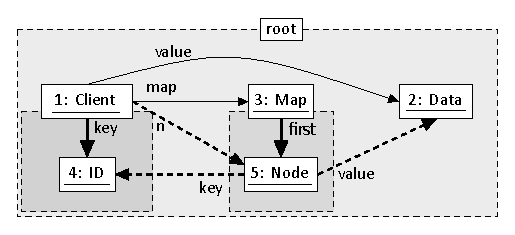
\includegraphics{ownership-dominator-vs-modifier.eps}
	\caption{Owners-as-Dominators vs. Owners-as-Modifiers}
	\label{fig:ownership-dominator-vs-modifier}
\end{figure}

\Cref{fig:ownership-dominator-vs-modifier}~\cite{dietl09gut} illustrates the 
difference between both encapsulation disciplines. References between objects 
are represented by arrows. The owner of an object is the class at the top of 
the dashed box the object is in.

If the \textbf{owner-as-dominator} discipline is adhered to, then only the 
solid arrows are allowed. The dashed arrows are references which do not pass 
through the object's owner, and as such are only allowed in the 
\textbf{owner-as-modifier} discipline. In the \textbf{owner-as-mod\-ifier} 
discipline, while such a reference is legal, these references cannot be used to 
mutate the state of the object being referenced.

\subsection{Applications}
\label{subsec:applications}

\subsubsection{Object Encapsulation}
\label{subsubsec:object_encapsulation}

Deriving directly from the example problem given in our 
\hyperref[code:modular_reasoning_car_engine_1]{introduction}, ownership types 
can be used to improve the expressibility of the concept of 
ownership~\cite{clarke98ownership}. This allows classes to restrict 
modification of their representation invariants by external code.

Therefore, when programmers are given a new code base annotated with ownership 
types, they can be ensured that no external code is able to modify the classes' 
invariants when they are understanding the code. This would allow them to 
locally reason about the function and behaviour of the module.

The same benefit would also apply for static analysis tools. Because changes 
can be effected only from one part of the program, a tool need only reason 
locally to form sound conclusions from the input. This would allow such tools 
to run in parallel on different parts of the program, allowing even complex 
analyses to scale with the size of the code base.

\subsubsection{Alias/Access Control}
\label{subsubsec:alias_control}

If programs adhere to the \textbf{owners-as-dominators} encapsulation 
discipline, then it is not possible to reference objects within another 
object's representation invariant. Therefore, aliases would be restricted to 
the scopes where references are 
allowed~\cite{clarke98ownership,boyapati04safejava,cameron07mojo}.

If programs adhere to the \textbf{owners-as-modifiers} encapsulation 
discipline, then there is not alias control; however, it is still not possible 
to modify the representation invariant of an object if the current object is 
not its owner~\cite{cunningham08ut,dietl09gut}.

In both cases, reasoning about side-effects are easy. In the former case, it is 
possible to increase the precision of alias analyses because aliasing is 
restricted to scopes where the reference is valid.

\subsubsection{Data Race/Deadlock Prevention}
\label{subsubsec:data_race_prevention}

Because ownership types impose a structure on the object store, it is possible 
to prevent data races. Typically, when an object A needs to be locked for an 
update, it is not obvious which dependent objects (references which A 
maintains) needs to be locked as well. Since there is an ownership topology 
imposed on the object store, it would be possible to know at compile-time which 
objects need to be locked as well, as part of locking A. This prevents data 
from being accessed, while accidentally forgetting to lock the object. Thus, 
data races can be prevented.

In the same vein, it is possible to prevent deadlocks from occurring by always 
locking a set of locks in the same order. Locking multiple locks in the same 
order prevents a circular wait condition, which is a necessary condition for a 
deadlock to occur~\cite{silberschatz08os}. Regardless of topology, 
locking objects using depth-first or breadth-first traversal guarantees that 
all objects which are reachable will be locked, and because the traversal is 
deterministic, will guarantee that the order of lock acquisition is always the 
same~\cite{boyapati02races}.

\subsubsection{Persisted Object Upgrades}
\label{subsubsec:object_upgrades}

Very often programs need to persist state to disk. The structure of this state 
might vary between versions of the same program. A problem is presented to the 
programmer: how to use the data (in the old format) in the updated program? 
Typically programmers will write transform functions which accept the old 
program state as input, and produces the corresponding new program state. This 
works well for simple objects; however, when the object graph is large, or 
contains cycles, the order to execute these transform functions may not be 
obvious.

Ownership types enforces a constraint on the structure object graph. This 
allows the programmer to write isolated transform functions that transforms 
only one type in the object graph. When used together with a transactional 
memory store, it is possible to individually transform objects in any order, so 
long all objects in the graph are eventually transformed. When the transaction 
is committed, it would be guaranteed that the new object graph would be 
valid statically~\cite{boyapati04safejava,boyapati03innerclass}.

\section{Variants}
\label{sec:variants}

In this section we give an overview of the four ownership type systems that we
have investigated in depth. The papers covered are by no means the entirety of
the work in the area. There are numerous other papers on extensions,
improvements and related developments~\cite{clarke13survey}. However we choose
these systems because they contributed important ideas and are (more or less)
representative of the gamut of work in ownership types. Each system will be
presented individually with a full cross-comparison provided in \cref{sec:eval}.

\subsection{Clarke's Ownership Types}
\label{subsec:clarke}

The concept of ``ownership'' was first introduced by Clarke et al. in his 1998
paper~\cite{clarke98ownership} with the motivation of mitigating the problems
of uncontrolled aliasing in Object-Oriented languages. This was a refinement of
a similar idea proposed by Clarke's thesis advisors called \emph{flexible alias
protection}~\cite{noble98alias} which, in turn, took inspiration from
Islands~\cite{hogg91islands} and Balloons~\cite{almeida97balloons}.

Islands and Balloons were early attempts at solving the same problem but did
not provide sufficient expressivity and ease-of-use to be practical. For
example, an object cannot be stored in two fully-encapsulated containers
simultaneously since a stored object would be considered a part of the
container's island/balloon and cannot be externally aliased. To mitigate this
problem, dynamic aliases (i.e.\ temporary stack-based references) into a
representation are permitted in both these works. Such aliases are read-only in
Islands, but have no restrictions in Balloons. Thus, while this ``escape
mechanism'' solves the problem, it can also expose the representation of the
container itself (e.g.\ nodes in a link-list) and provide no encapsulation in
the case of Balloons. Moreover, the authors of~\cite{noble98alias} argue that
it would be hard for programmers to use Balloons because of the complex
abstract interpretation required.

Ownership types solve the problem by providing a more flexible/intuitive syntax
to the programmer for defining a hierarchical topology over objects without
sacrificing encapsulation. The idea is to annotate types with modifiers
that define which context (i.e.\ owner) each reference belongs to, which
include: \vspace{-1ex}
\begin{itemize}
	\setlength\itemsep{-0.2ex}
	\item \textbf{\lstinline|norep|}:
		Not part of the representation of any object.
	\item \textbf{\lstinline|rep|}:
		Owned by \lstinline|this| object and is part of its representation.
	\item \textbf{\lstinline|owner|}:
		Owned by the owner of \lstinline|this| object.
	\item \textbf{$v$}:
		A context parameter.
\end{itemize} \vspace{-1ex}

Context parameters are declared on classes with a syntax similar to Java's
generics, e.g. \lstinline|class List<t> { ... }|, and are similarly applied on
types, e.g. \lstinline|rep List<norep> list;|. They allow owners higher in the
hierarchy to declare their ownership of references held by descendants in their
contexts. In the case of the previous \lstinline|list| example, the
\lstinline|list| is declared to be part of the client object's context, but the
elements it contains has no owner. Parameterized ownership is the key
innovation that (partially) solves the container problem and also enables
different roles for different references of the same object class.

These declarations and parameters describe a hierarchical structure of object
representations that can be easily verified at compile-time. If well-typed, the
programmer can be assured of that there can be no external aliases to any of
the objects within a particular context, guaranteeing encapsulation. In
particular, Clarke's ownership types enforces the \emph{owners-as-dominators}
discipline, which ensures that all paths to an object must pass through its
owner.

However, ownership types as originally presented in~\cite{clarke98ownership}
still had limitations. For example, rules for inheritance/subtyping were yet to
be developed and the encapsulation discipline was still too strict to be of
practical use (e.g.\ iterators are not possible). Addressing these and other
limitations was the main focus of subsequent work on the subject, a few of
which are covered in the following sections~\cite{boyapati04safejava,
boyapati03innerclass, cunningham08ut, dietl11gut, cameron07mojo}.

% Iterators not possible (too strict because of owners-as-dominators discipline)
% - In XStack example, iterator modification has to go through stack
%
% - Iterator is only usable in the context of the owner of both the iterator and
%	 stack
%
% - Boyapati: A type system that strictly enforces object encapsulation is 
%	 too constraining [113]: it does not allow efficient implementation of
%	 important constructs like iterators [104, 71]. Consider, for example, an
%	 iterator over the above-mentioned Stack object s. If the iterator is
%	 encapsulated within s, it cannot be used outside s. If the iterator is not
%	 encapsulated within s, it cannot directly access the list nodes in s, and
%	 hence cannot run efficiently. [SafeJava, pg 25]
%
% Multiple owners not possible
% - Cannot append two XStacks together because an append() function would have
% to be declared rep. The other xstack would have a problem to be passed to the
% first xstack because the contexts are different
%
% Not possible to transfer ownership
% - Example?
%
% No inheritance; Inheritance not supported (or just not discussed)
%
% Key Idea: Ownership types impose structural invariants on the object graphs of
% well-typed programs that limit the kinds of aliasing possible
% - e.g. getter functions which return references to objects within the
%	 invariant, allowing internals to be modified outside the owner.


\subsection{Boyapati's SafeJava}
\label{subsec:boyapati}



% For solving the iterator problem
%
% Fully parametized ownership type system (conflicts with Java’s generics
% syntax) with constraints (e.g. where sOwner <= tOwner)
%
% Does not have rep or norep keywords → uses this and world on first parameter
% of object reference to denote primary owner.
%
% Supports effects clauses and constraints.
%
% Supports inheritance
%
% Support ownership transfer
% only for unique references. unique references can be ‘borrowed’ so that in
% a local scope an alias exists. Not completely static. (p54) Leaves null
% pointers at runtime.
%
% Key Idea: Inner-classes (or classes in the same ‘module’) have privileged
% access to the representation of the enclosing class -- ownership structure
% unchanged, only access rules modified with an exception for inner-classes. The
% concept of a peer in Universes seems to generalize this.
%
% - Ownership types can be mostly verified at compile time, but dynamic casts
% are allowed in Java and so he proposes a complementary runtime system that
% checks casts.
%
% Secondary owners must necessarily be ancestors of the primary owner. This is
% because users parameterising the class would not know of any descendents of
% the primary owner due to the encapsulation barrier.




\subsection{Dietl and M\"{u}ller's Universe Types}
\label{subsec:dietl}

% Uses modifiers rep, peer, any on references, and pure/impure on methods.
%
% Additional modifiers self and lost are never used when annotating source code,
% but are required in the type system for checking. 
% - lost is denotable but not expressible, more information than any (that’s why
%	  we can cast lost -> any). Assigning to lost fields is a type error.
% - any is denotable and expressible. Fields of type any can be assigned to
%
% The peer modifier is distinct from owner in the original paper. Peer means
% that the referenced object is a co-owner of the representation, owner means
% that the reference object has the same owner (but does not have representation
% access). In this sense, universes allow primitive support for multiple owners,
% as long as these ‘peers’ are declared in the same module.
%
% Vanilla Universe Types requires runtime checking without parameterization. An
% example is the use of any for references to values in a container class. This
% implies that the references are read-only --- the user of a container cannot
% obtain and modify the objects with these read-only references UNLESS they are
% casted to rep something, with the appropriate runtime check. Generic Universe
% Types solves this problem.
%
% Iterators can be more efficient because they can have direct access to the
% representation of the container for reading and writing.


\subsection{Cameron's Multiple Ownership}
\label{subsec:cameron}

% Key idea: dropping the owner-as-dominator requirement and allowing multiple
% owners gives more expressiveness at the cost of the looser guarantees
% - Classical ownership: owners-as-dominators/modifiers; solution is to flatten
%   ownership structures
% - DAG object topologies are more expressive than the traditional trees
% - Guarantees now relate to computational effects, not encapsulation
% - Modifier guarantee unchanged
%
% Ownership wildcards/basic existential quantification (one owner not knowing
% details of others)
%
% intersects and disjoint (helps control effects as well) constraints which
% limit possible multiple ownership
%
% where clauses for ownership parameters

\lipsum[10]



\section{Evaluation}
\label{sec:eval}

\lipsum[11]




\section{Conclusion}
\label{sec:conclude}

% Need dynamic checking of ownership if casting or reflection is possible
% - In practice, compile-time checking alone is insufficient

% Annotations are a burden on programmers
% - Declare everything to be owned by root/world?
% - Limits of ownership inference?



\lipsum[12]

\begin{table*}[t]
\caption{Expressivity and (Analytical) Benefits of Ownership Type Systems}
\label{tab:summary}
\centering
\NewDocumentCommand{\rot}
	{O{45} O{1.8em} m}{\makebox[#2][l]{\rotatebox{#1}{#3}}}
\newcommand{\Yes}{$~\medbullet$}
\newcommand{\Limited}{$~\medcirc$}
\newcommand{\Maybe}{$~\bigtriangleup$}
\newcommand{\No}{$~\times$}
\newcommand{\note}[1]{\textsuperscript{$#1$}}
\newcommand{\comment}[2]{
	& & \multicolumn{12}{l}{
		\scriptsize \note{#1}\,#2 \vspace{-0.7em}
	} \\
}
\renewcommand{\arraystretch}{1.4}
\vspace{1em}
\begin{tabular}{rllllllllllllll}
	\scriptsize
	\begin{tabular}[b]{|rl|} \hline
		\Yes & Supported \\	
		\Limited & Partially Supported \\
		\No & Not Supported   \\
		\Maybe & Not Discussed \\
		\hline \multicolumn{1}{r}{}
	\end{tabular} \hspace{10pt}
&~&
\rot{Immutable View} &
\rot{Mutable View} &
\rot{Binary Operations} &
\rot{Class Inheritance} &
\rot{Ownership Constraints} &
\rot{Ownership Transfer} &
\rot{Generic Ownership} &
\rot{Generic Types} &
\rot{Multiple Owners} &
\rot{\bf Alias Control} &
\rot{\bf Effect Specifications} &
\rot{\bf Local Reasoning} &~~
\\ \toprule
Ownership Types~\cite{clarke98ownership}&
	& \No & \No & \No & \Maybe & \No & \No & \Yes & \Maybe & \No
	& \Yes & \Maybe & \Yes
\\ 
SafeJava~\cite{boyapati04safejava}&
	& \Yes & \Yes & \No & \Yes & \Yes & \Yes & \Yes & \Maybe & \No
	& \Yes & \Yes & \Yes
\\
Universe Types~\cite{cunningham08ut}&
	& \Yes & \No & \Yes & \Yes & \No & \Maybe & \No & \Maybe & \No
	& \No & \Limited\note{\ast} & \Yes
\\
Generic Universe Types~\cite{dietl11gut}&
	& \Yes & \No & \Yes & \Yes & \No & \Maybe & \Yes & \Yes & \No
	& \No & \Limited\note{\ast} & \Yes
\\
Multiple Ownership~\cite{cameron07mojo}&
	& \Yes & \Yes & \Yes & \Yes & \Yes & \Maybe & \Yes & \Maybe & \Yes
	& \Yes & \Yes & \Limited\note{\dagger}
\\ \bottomrule
\comment{\ast}{
	UT/GUT only supports \lstinline|pure| and \lstinline|impure|, rather than
  the more general \lstinline|reads| and \lstinline|writes| declarations.
}
\comment{\dagger}{
	The ownership wildcard \lstinline|?| limits the local reasoning possible.
}
\end{tabular}
\end{table*}






\section{Testing}
\label{sec:test}

% Code Snippets
\begin{lstlisting}[
	float, floatplacement=t,
	caption={Car Engine Example},
	label=code:car_eng_test
]
class Person {}
class Engine<any engineOwner> {
  pure void start() { /* ... */ }
}

class Car<carOwner, driverOwner> {
  rep Engine<this> engine;
	norep Person<a & ?> driver;
    
  impure void start() {
    if (driver != null) getEngine().start();
  }
  Engine<world> getEngine() reads { return engine; }
}
\end{lstlisting}

% Figures
\begin{figure}[t]
\centering
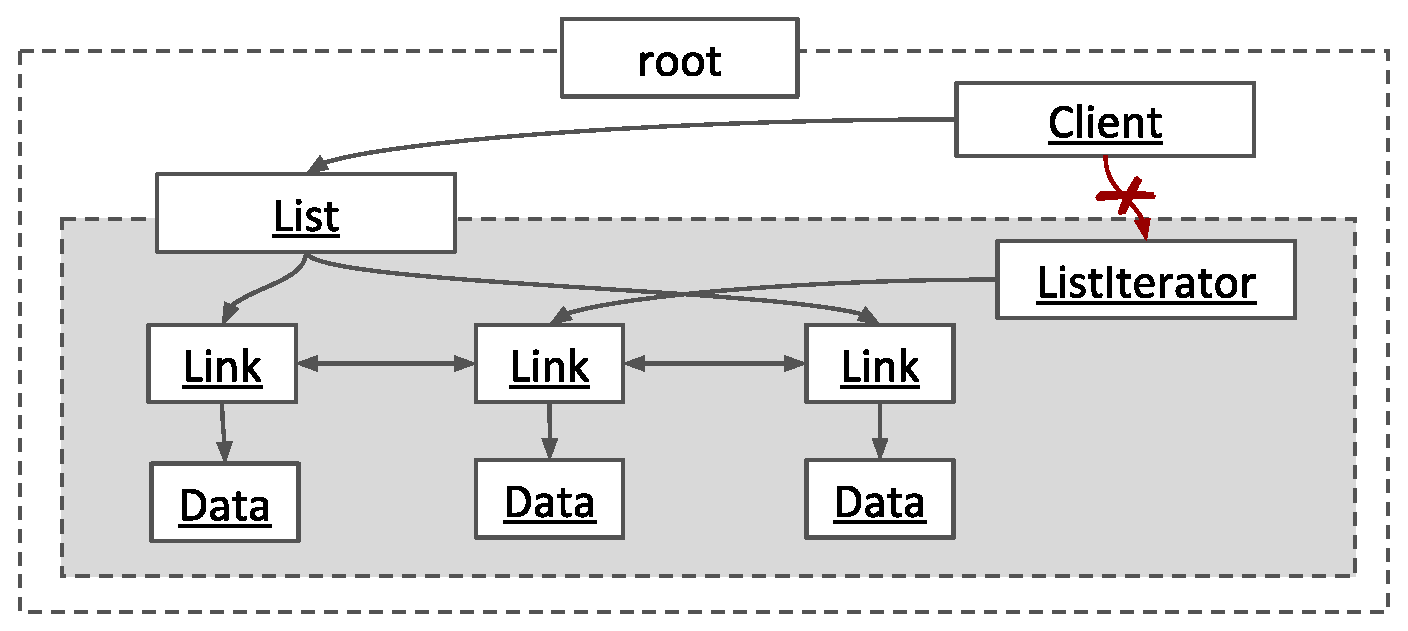
\includegraphics{iterator-fail-inside.eps}
\caption{List Iterator inside representation.}
\label{fig:iterator-inside-test}
\end{figure}

\begin{figure}[t]
\centering
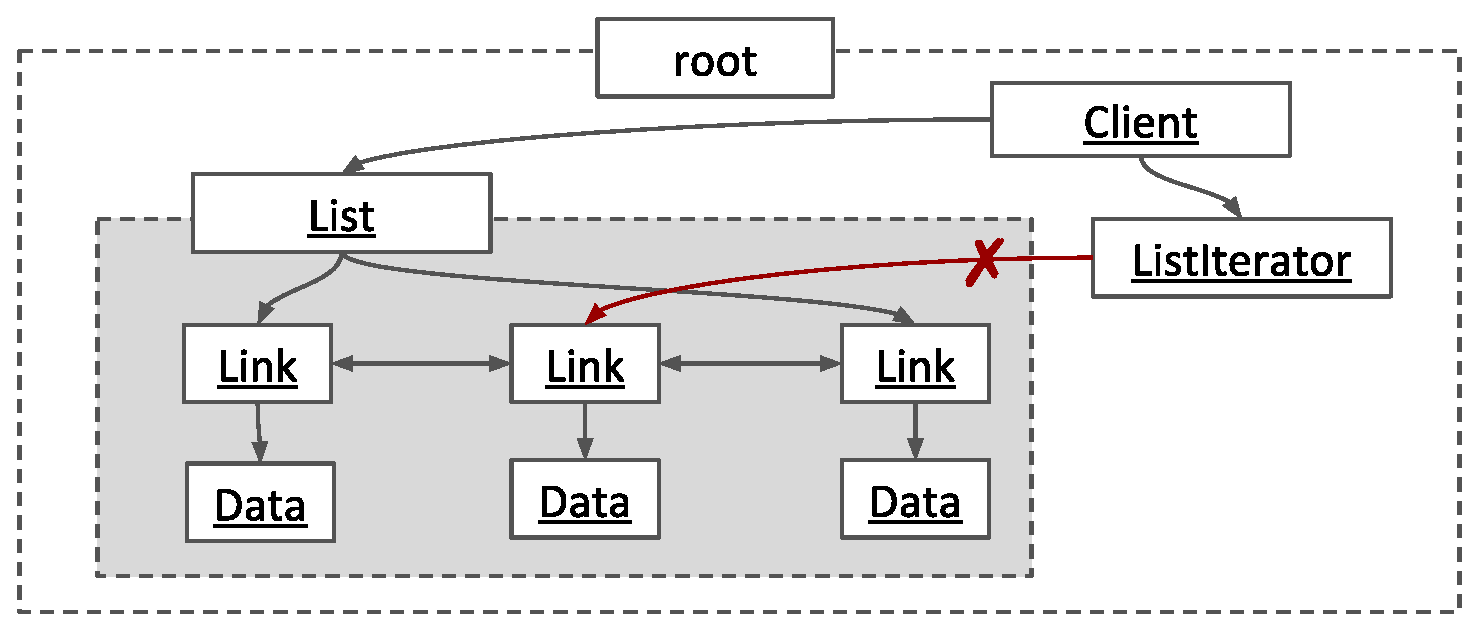
\includegraphics{iterator-fail-outside.eps}
\caption{List Iterator outside representation.}
\label{fig:iterator-outside-test}
\end{figure}

Reference to \cref{code:car_eng_test}, \cref{sec:test} and 
\cref{fig:iterator-inside-test,fig:iterator-outside-test}.

% Citations
aldrich04domains~\cite{aldrich04domains},\newline
aldrich02aliasjava~\cite{aldrich02aliasjava},\newline
almeida97balloons~\cite{almeida97balloons},\newline
boyapati04safejava~\cite{boyapati04safejava},\newline
boyapati02races~\cite{boyapati02races},\newline
boyapati03innerclass~\cite{boyapati03innerclass},\newline
boyapati03rtsj~\cite{boyapati03rtsj},\newline
cameron07mojo~\cite{cameron07mojo},\newline
cameron10encoding~\cite{cameron10encoding},\newline
clarke03ownership~\cite{clarke03ownership},\newline
clarke02ownership~\cite{clarke02ownership},\newline
clarke13aliasing~\cite{clarke13aliasing},\newline
clarke98ownership~\cite{clarke98ownership},\newline
cunningham08ut~\cite{cunningham08ut},\newline
dietl09gut~\cite{dietl09gut},\newline
dietl11gut~\cite{dietl11gut},\newline
dietl07gut~\cite{dietl07gut},\newline
dietl13ownership~\cite{dietl13ownership},\newline
dietl08dependent~\cite{dietl08dependent},\newline
dietl05jml~\cite{dietl05jml},\newline
hogg91islands~\cite{hogg91islands},\newline
muller02modular~\cite{muller02modular},\newline
muller99universes~\cite{muller99universes},\newline
noble98alias~\cite{noble98alias}, \newline
clarke13survey~\cite{clarke13survey}



\bibliographystyle{abbrv}
\bibliography{report}

\end{document}
